\section{Quantum entanglement}\label{sec:quantum-entanglement}
The fundamental goal is to use entangled states to conduct optical test of Q.M., but we need to have single photons in order to conduct interference experiments and teleportation.
In Q.M. the observables follow a probability distribution and unless a system is in a eigenvalue of the observable, all we can do is to predict the probability with a particular eigenvalue when the measurement is repeated several times on identically prepared systems.

This means that making a measurement \textbf{doesn't reveal a pre-existing value of the observable}. The act of measurement makes the wave function collapse in a way that is not certain.

Suppose to prepare a photon as bit 1 in $\ket{V}$ state, a measurement of the diagonal component $\ket{D_+}$ with a beam splitter could return the value $+1$ (transmission) or $-1$ (reflection) with equal probability $50 \%$.
Until the measurement is made it simply doesn't have a well defined value of the diagonal component. This reflect the \textbf{orthodox view of Q.M.}

Instead, the \textbf{realist position} consider the Q.M. as an incomplete theory requiring some other unknown information to complete the description of the physical system. This lead to the \textbf{Hidden variables theory and EPR paradox 1935}.
\subsection{EPR-B}
Now we discuss a simplified version of EPR proposed by Bohm:

Let us assume to have  a source that emits photon pairs having \textbf{correlated polarizations}, if one is $\ket{H}$ the other one will be $\ket{V}$. We can describe it with the following form:
\begin{equation}\label{eqn:15-entangled-state-example}
\ket{\psi} = \frac{1}{\sqrt{2}} \,  \bigl(\ket{H,V}-\ket{V,H}\bigr)
\end{equation}

the photons are indistinguishable, each on can be equally $\ket{H}$ and $\ket{V}$. This configuration is a classic example of an \textbf{entangled state:} a name reserved to states that cannot be expressed as tensor product states $\ket{H}\otimes  \ket{V}$.

Suppose two photons are emitted in opposite directions, then we place a B.S. and a photodetector at $10$ m far from the source and measure one of the photons and obtain $\ket{H}$. We immediately know -- even at any arbitrary distance -- that the other photon measurement, performed by a trusted friend of us, will get $\ket{V}$.

In the \say{realist} point of view: the distant photon our friend measured was always $\ket{V}$, since the moment it was emitted. Instead, in the \say{orthodox} point of view: the measurement collapses the wave function and produces instantaneously the state $\ket{H}$ for one photon and $\ket{V}$ for the other one. This seems to contradict the relativistic principle: information can't travel faster than light.

% / / / / / / / / / / / / / / / / / / / / / / / / / / / / / / / / / / / / / / / /
% / / / / / / / / / / / / / / / / / / / / / / / / / / / / / / / / / / / / / / / /

\callouterror{%
\subsection{Bell experiment}
Allowed two polarizers to be independently adjusted (da capire). We have a polarizer A with $\vec{n}_A$ orientation and a polarizer B with $\vec{n}_B$ orientation. He proposed to compute the average of the product of the polarizations for a given pair of correlated photons and polarizers  orientation.

According to Q.M.
\[P(\vec{n}_A,\vec{n}_B) = -\vec{n}_A\cdot\vec{n}_B\]

Bell demonstrate that this result is incompatible with any local hidden variable theory. If we suppose to have a third polarizer $\vec{n}_C$, it is possible to derive the \textbf{Bell inequality}
\[
|P(\vec{n}_A,\vec{n}_B)-P(\vec{n}_A,\vec{n}_C)| \leq 1+ P(\vec{n}_B,\vec{n}_C)
\]
And it holds for any local hidden variable theory. Q.M. turns out to be incompatible with Bell's inequality, to show this suppose to have three polarization directions such as: 
\begin{figure}[H]
    \centering
    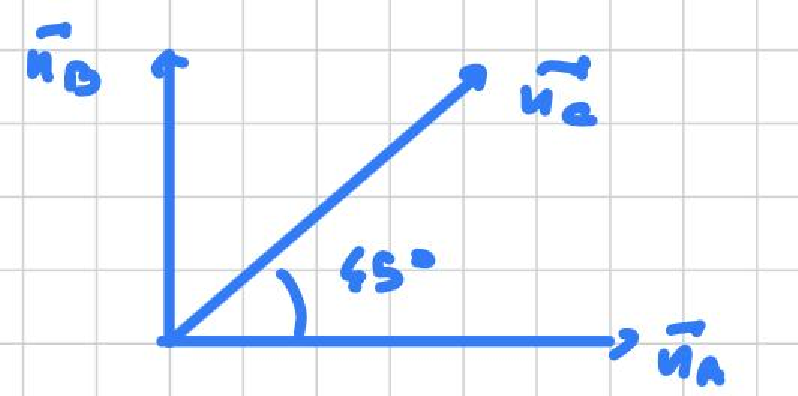
\includegraphics[width=0.6\linewidth]{images_in_pdf/15-/Grafico_82.pdf}
\end{figure}

\[P(\vec{n}_A,\vec{n}_B) =-\vec{n}_A\cdot \vec{n}_B =0 \hspace{1cm} P(\vec{n}_A,\vec{n}_C) = P(\vec{n}_B,\vec{n}_C) = -\frac{\sqrt{2}}{2} = -0.707\]

It can be easily shown that is inconsistent with Bell's inequality:
\[|0-\frac{\sqrt{2}}{2}| \leq 1-\frac{\sqrt{2}}{2} \implies \frac{\sqrt{2}}{2} \cancel{\leq} 1-\frac{\sqrt{2}}{2}\]
if the inequality is not satisfied, Q.M. is correct and hidden variable theory doesn't hold.

\textbf{Experimental test:} suppose to have a structure as 
\begin{figure}[H]
    \centering
    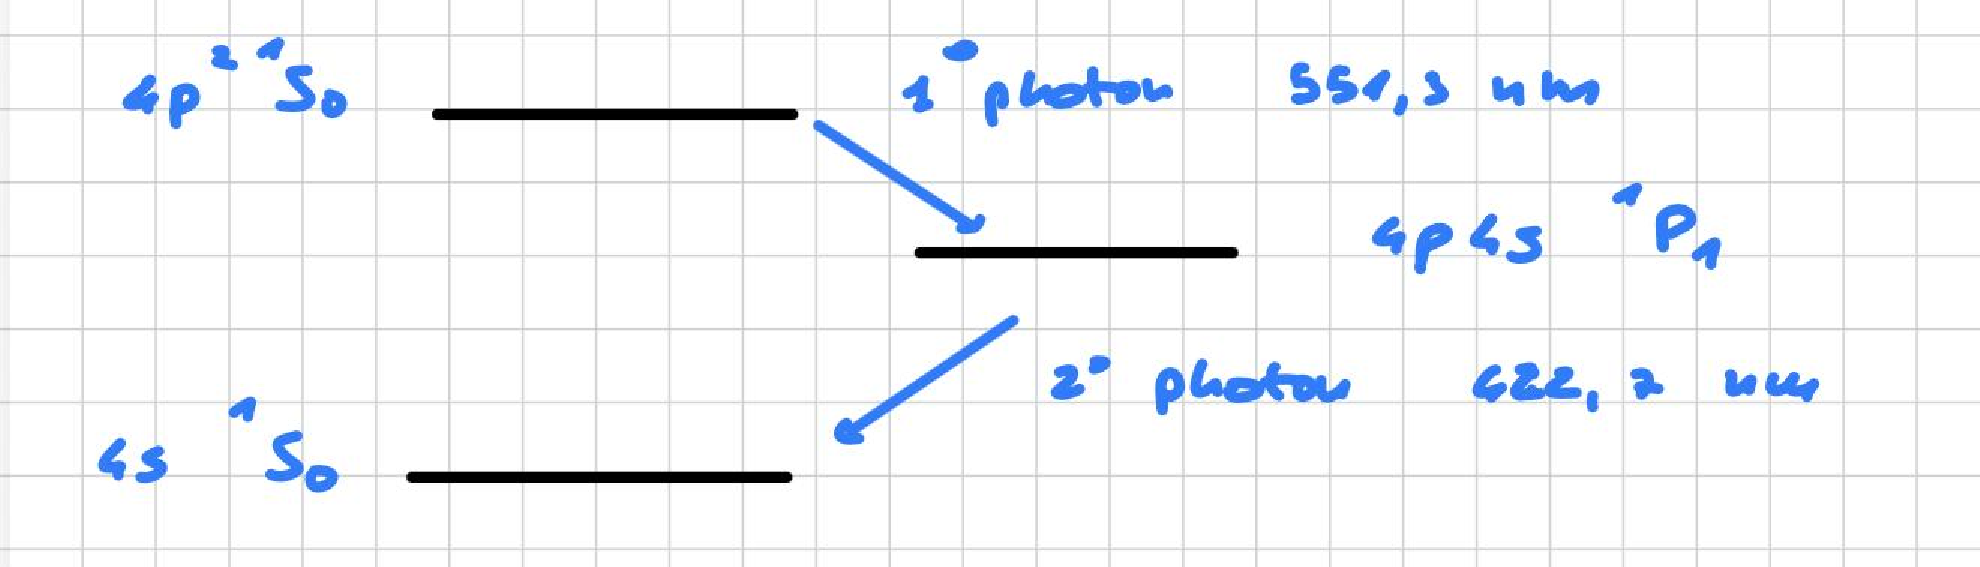
\includegraphics[width=0.6\linewidth]{images_in_pdf/15-/Grafico_83.pdf}
\end{figure}

\begin{itemize}
    \item The ground state and the excited state are $J=0$ states, which means that photon pairs have no net angular momentum.

    \item The parity of the energy levels implies polarization correlation.
\end{itemize}

The set up consists in a beam of $Ca$ atoms which is excite, this generates a pair of photons propagating in opposite directions, each one goes to a PM polarimeter (that measure the linear polarization), a filter $F_i$ (to select photon wavelengths) and then a PMT photomultiplier. Both the photomultipliers are connected to a same electronic system.
\begin{figure}[H]
    \centering
    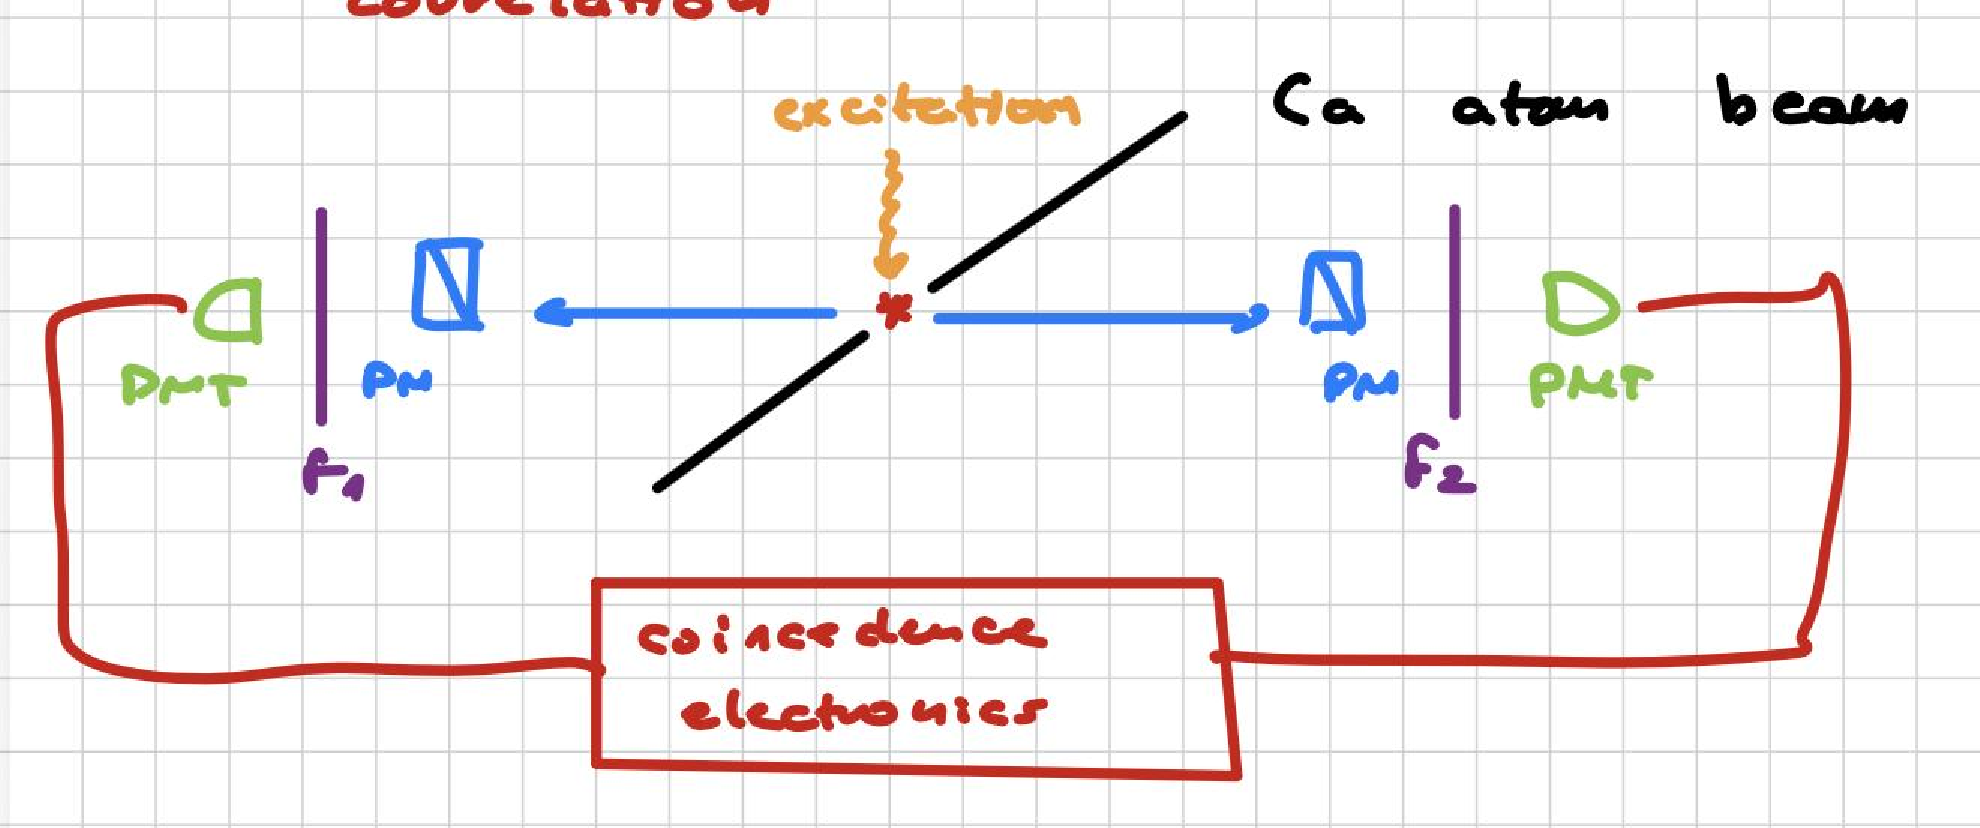
\includegraphics[width=0.6\linewidth]{images_in_pdf/15-/Grafico_84.pdf}
\end{figure}

if we measure along $\vec{n}_A$ direction, this yields to $\ket{V}$ if the polarization is parallel to $\vec{n}_A$ or $\ket{H}$ if the polarization is perpendiculare to $\vec{n}_A$. We can define the \textbf{correlation coefficient:}
\[E(\vec{n}_A,\vec{n}_B) = P_{VV}(\vec{n}_A,\vec{n}_B)+P_{HH}(\vec{n}_A,\vec{n}_B)-P_{VH}(\vec{n}_A,\vec{n}_B)-P_{HV}(\vec{n}_A,\vec{n}_B)\]

Let us consider a combination for two different orientations $(\vec{n}_A,\vec{n}_A')$ and $(\vec{n}_B,\vec{n}_B')$ of the polarizers:
\[S = E(\vec{n}_A,\vec{n}_B)-E(\vec{n}_A',\vec{n}_B')+ E(\vec{n}_A,\vec{n}_B')+E(\vec{n}_A',\vec{n}_B)\]

In realistic local theory view the Bell inequality reads:
\[-2\leq S\leq 2\]
Instead according to Q.M. for particular orientations of $(\vec{n}_A,\vec{n}_A')$ and $(\vec{n}_B,\vec{n}_B')$, we can obtain:
\[S = \pm 2\sqrt{2}\]
this result contradicts the Bell inequality called \textbf{CSCH inequality}.

If we choose a orientation such that:
\[\vec{n}_A\cdot\vec{n}_B = \vec{n}_A'\cdot\vec{n}_B = \vec{n}_A'\cdot\vec{n}_B' = \cos(\theta) \hspace{1cm} \vec{n}_A\cdot\vec{n}_B' = cos(3\theta)\]

We obtain:
\[S = 3\cdot \cos(2\theta)-\cos(6\theta)\]

it is possible to see that for $0\leq \theta \leq 90$ there are some values of S that violate the Bell's inequality, this show us the M.Q. prediction with:
\[S = 2.697\pm 0.015 \hspace{1cm} \theta = \qty{22.5}{\degree}\]

\begin{figure}[H]
    \centering
    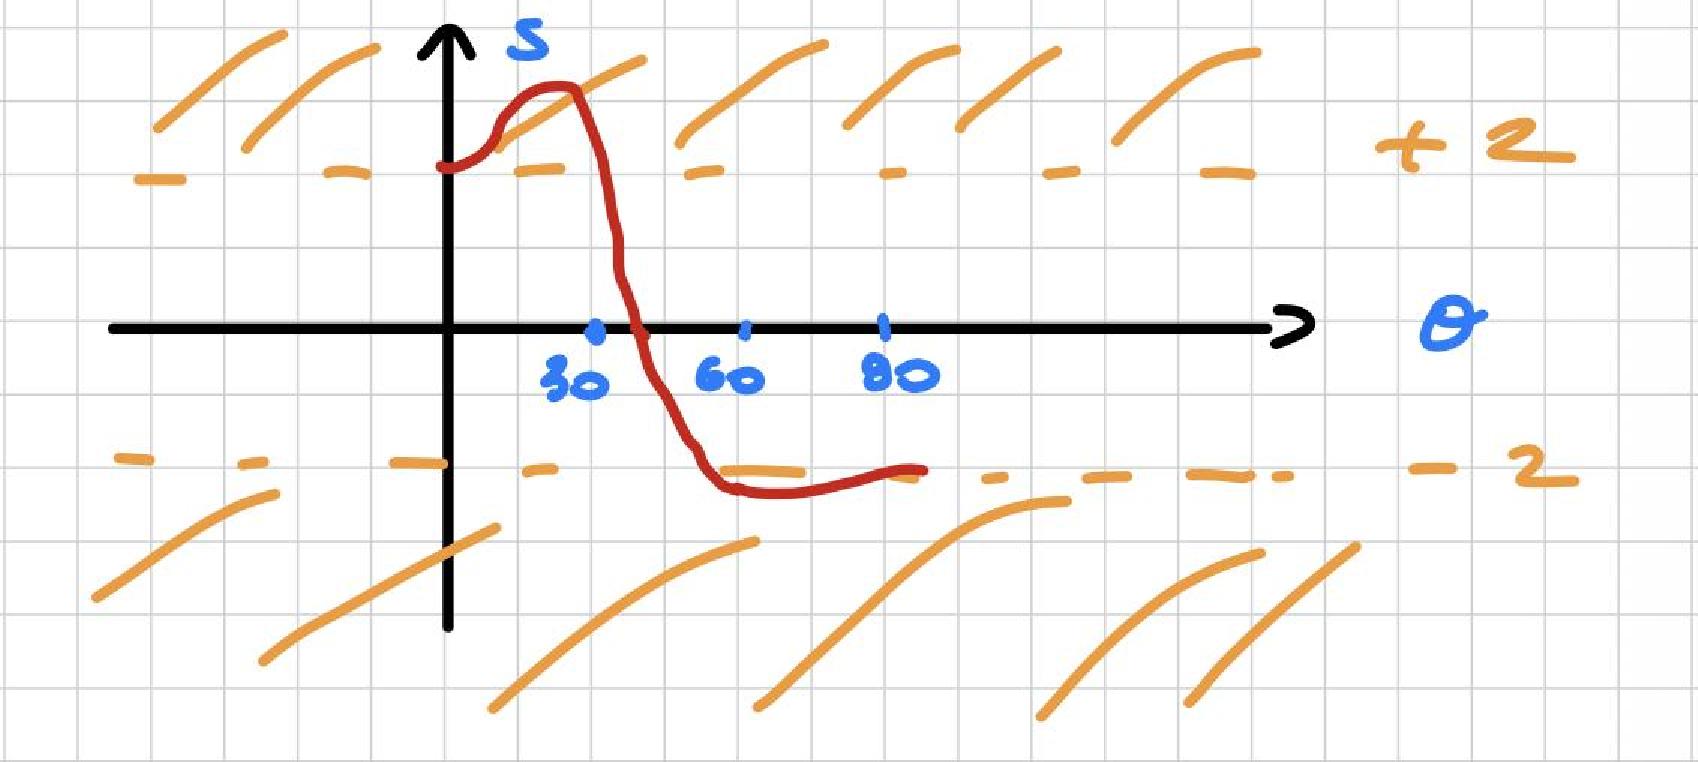
\includegraphics[width=0.6\linewidth]{images_in_pdf/15-/Grafico_85.pdf}
\end{figure}

One must also consider the \textbf{loop-hole problem}. In principle, there is always a possibility that the two measurement stations exchange information during the experiment. To suppress this possibility, the setup can be improved by adding two more photomultipliers and two acousto-optic devices, which change the refractive index of the crystal through sound waves driven by a transducer. The switching time is about $20\,\mathrm{ns}$, which is much smaller than the light travel time between the two stations, $\Delta t \ll L/c$, where $L$ is the distance between the polarizers.

Other possible loopholes are:
\begin{itemize}
    \item \textbf{Freedom-of-choice loophole:} the orientation settings of the analyzers must be chosen independently of the properties of the particle pair.
    
    \item \textbf{Detection loophole:} only a subset of the emitted pairs is detected, so one could argue that the recorded events are not representative of the whole ensemble. This loophole is closed only when the detection efficiency is sufficiently high, typically around $\eta \approx 83\%$ in the standard CHSH scenario.
\end{itemize}

A fully loophole-free experimental demonstration was achieved in 2015 using advanced quantum technologies.

Bell's result does not show that faster-than-light signals exist, but rather that no theory based on \textbf{local hidden variables} can reproduce all the quantum predictions. In a local hidden-variable model, each photon in an entangled pair is assumed to carry predetermined local properties before the measurement is performed. Bell derived an inequality that any such theory must satisfy, and experiments have repeatedly violated this inequality. 
This means that the state of the system is not fully encoded in pre-existing local properties before the measurement.
}

% / / / / / / / / / / / / / / / / / / / / / / / / / / / / / / / / / / / / / / / /
% / / / / / / / / / / / / / / / / / / / / / / / / / / / / / / / / / / / / / / / /

\subsection{Bell experiment}

The core of John Bell's theorem relies on a setup where the orientation of two distant polarizers can be adjusted completely independently. Let polarizer A be oriented along the direction $\vec{n}_A$ and polarizer B along $\vec{n}_B$. Bell proposed to evaluate the statistical correlation between the two measurement stations by computing the expectation value (average) of the product of the polarization outcomes for a given pair of entangled photons.

According to quantum mechanics, the correlation function for a polarization-entangled singlet-like state is given by:
\begin{equation}\label{eqn:15-quantum-correlation}
P(\vec{n}_A,\vec{n}_B) = -\vec{n}_A\cdot\vec{n}_B.
\end{equation}

Bell demonstrated that this quantum mechanical result is fundamentally incompatible with any local hidden-variable (LHV) theory. By introducing a third alternative polarizer orientation $\vec{n}_C$, one can derive the classic \textbf{Bell inequality}:
\begin{equation}\label{eqn:15-bell-inequality}
|P(\vec{n}_A,\vec{n}_B)-P(\vec{n}_A,\vec{n}_C)| \leq 1 + P(\vec{n}_B,\vec{n}_C),
\end{equation}
which must strictly hold for any LHV model. To prove that quantum mechanics violates this constraint, let us select three specific coplanar polarization directions separated by $45^\circ$, such that:

\begin{figure}[H]
    \centering
    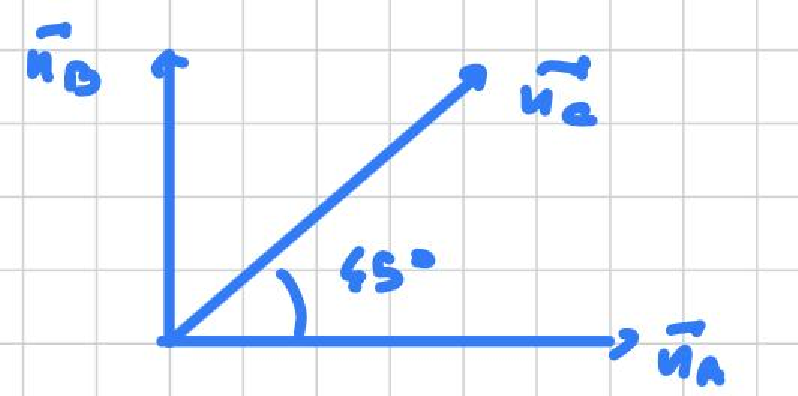
\includegraphics[width=0.6\linewidth]{images_in_pdf/15-/Grafico_82.pdf}
\end{figure}

Evaluating the quantum mechanical correlations yields:
\[
P(\vec{n}_A,\vec{n}_B) =-\vec{n}_A\cdot \vec{n}_B = 0, \qquad P(\vec{n}_A,\vec{n}_C) = P(\vec{n}_B,\vec{n}_C) = -\cos(45^\circ) = -\frac{\sqrt{2}}{2} \approx -0.707.
\]

Substituting these values directly into Bell's inequality leads to an explicit contradiction:
\[
\left|0 - \left(-\frac{\sqrt{2}}{2}\right)\right| \leq 1 + \left(-\frac{\sqrt{2}}{2}\right) \implies \frac{\sqrt{2}}{2} \not\leq 1 - \frac{\sqrt{2}}{2},
\]
since $0.707 \not\leq 0.293$. This geometric violation formally proves that quantum mechanics cannot be reproduced by any local deterministic hidden-variable framework.

\callout{Uselessy formal discussion of the CHSH inequality violation}{%

Suppose Alice and Bob are two observers who can independently choose between two measurement settings, denoted as $a$ and $a'$ for Alice, and $b$ and $b'$ for Bob. All these measurements have the same possible outcomes: $\pm 1$. Each one of them has access to one out of two correlated particles. 
\begin{equation}\label{eqn:15-chsh-scheme}
\begin{aligned}
&\text{Alice measures}\quad &&\text{Bob measures} \\
&a, a' = \pm 1 && b, b' = \pm 1\\
\end{aligned}
\end{equation}

We can introduce a derived observable $C$ defined as:
\begin{equation}\label{eqn:15-chsh-observable}
    C = (a+a')b + (a-a')b'
\end{equation}

which, by construction, can only take the values $\pm 2$:
\begin{equation}\label{eqn:15-chsh-values}
\begin{cases}
    a   =  a' \implies a+a' = \pm2,\ a-a'=0\\
    a \neq a' \implies a+a' = 0,\ a-a' = \pm2
\end{cases}
\implies
C = \pm 2,\ \forall\, a, a', b, b'.
\end{equation}

for any observable, it must hold that:
\begin{equation}\label{eqn:15-triangular-inequality}
    |\braket{C}| \leq \braket{|C|} 
\end{equation}

since $|C|=2$, we find the CHSH inequality:
\begin{equation}\label{eqn:15-chsh-inequality}
    |\braket{C}| \leq 2.
\end{equation}

in the photonic picture, the observables $a$ and $a'$ can be seen as polarization measurements in two different basis (e.g. horizontal-vertical or diagonal plus-minus); same applies for $b$ and $b'$. 

We now show that quantum mechanics predicts a violation of the CHSH inequality. 
\begin{proof}

Suppose that the couples of particles shared by Alice and Bob are prepared in a maximally entangled state, such as the singlet state:
\begin{equation}\label{eqn:15-singlet-state}
    \ket{\psi} = \frac{1}{\sqrt{2}} \,  \bigl(\ket{0,1}-\ket{1,0}\bigr).
\end{equation}

where $\ket{0}$ and $\ket{1}$ are eigenvectors of any couple of the observables measurable by Alice and Bob. There's no need to be more specific than this.

\end{proof}
}


\subsubsection{Experimental test} 
To test this prediction in the laboratory, one can exploit an atomic cascade source. Consider a calcium (\ce{Ca}) atom characterized by the following energy-level structure:

\begin{figure}[H]
    \centering
    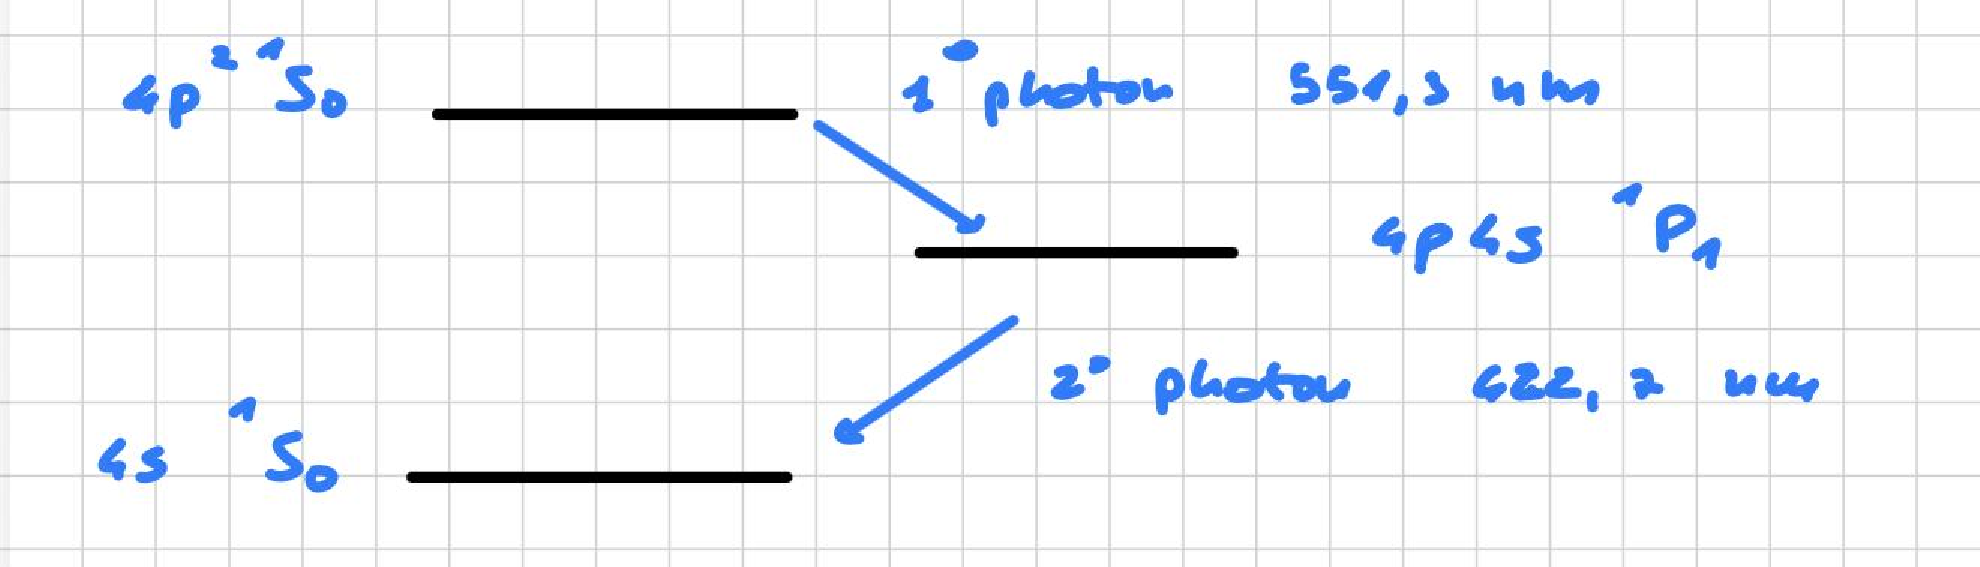
\includegraphics[width=0.6\linewidth]{images_in_pdf/15-/Grafico_83.pdf}
\end{figure}

\begin{itemize}
    \item Both the ground state and the excited state are $J=0$ angular momentum states, meaning the \hl{emitted photon pairs carry no net total angular momentum};
    \item The well-defined parity of these energy levels enforces a strict polarization correlation between the two photons to conserve total angular momentum.
\end{itemize}

The experimental setup consists of a calcium atomic beam excited via a two-photon process. The subsequent cascade decay generates a pair of entangled photons propagating in opposite directions. Each photon is directed toward a measurement arm containing a wavelength filter $F_i$ (to isolate the respective cascade transition), a linear polarimeter to analyze the polarization along $\vec{n}_i$, and a high-sensitivity photomultiplier tube (PMT). Both PMTs are connected to a central coincidence electronics system to register simultaneous detection events.

\begin{figure}[H]
    \centering
    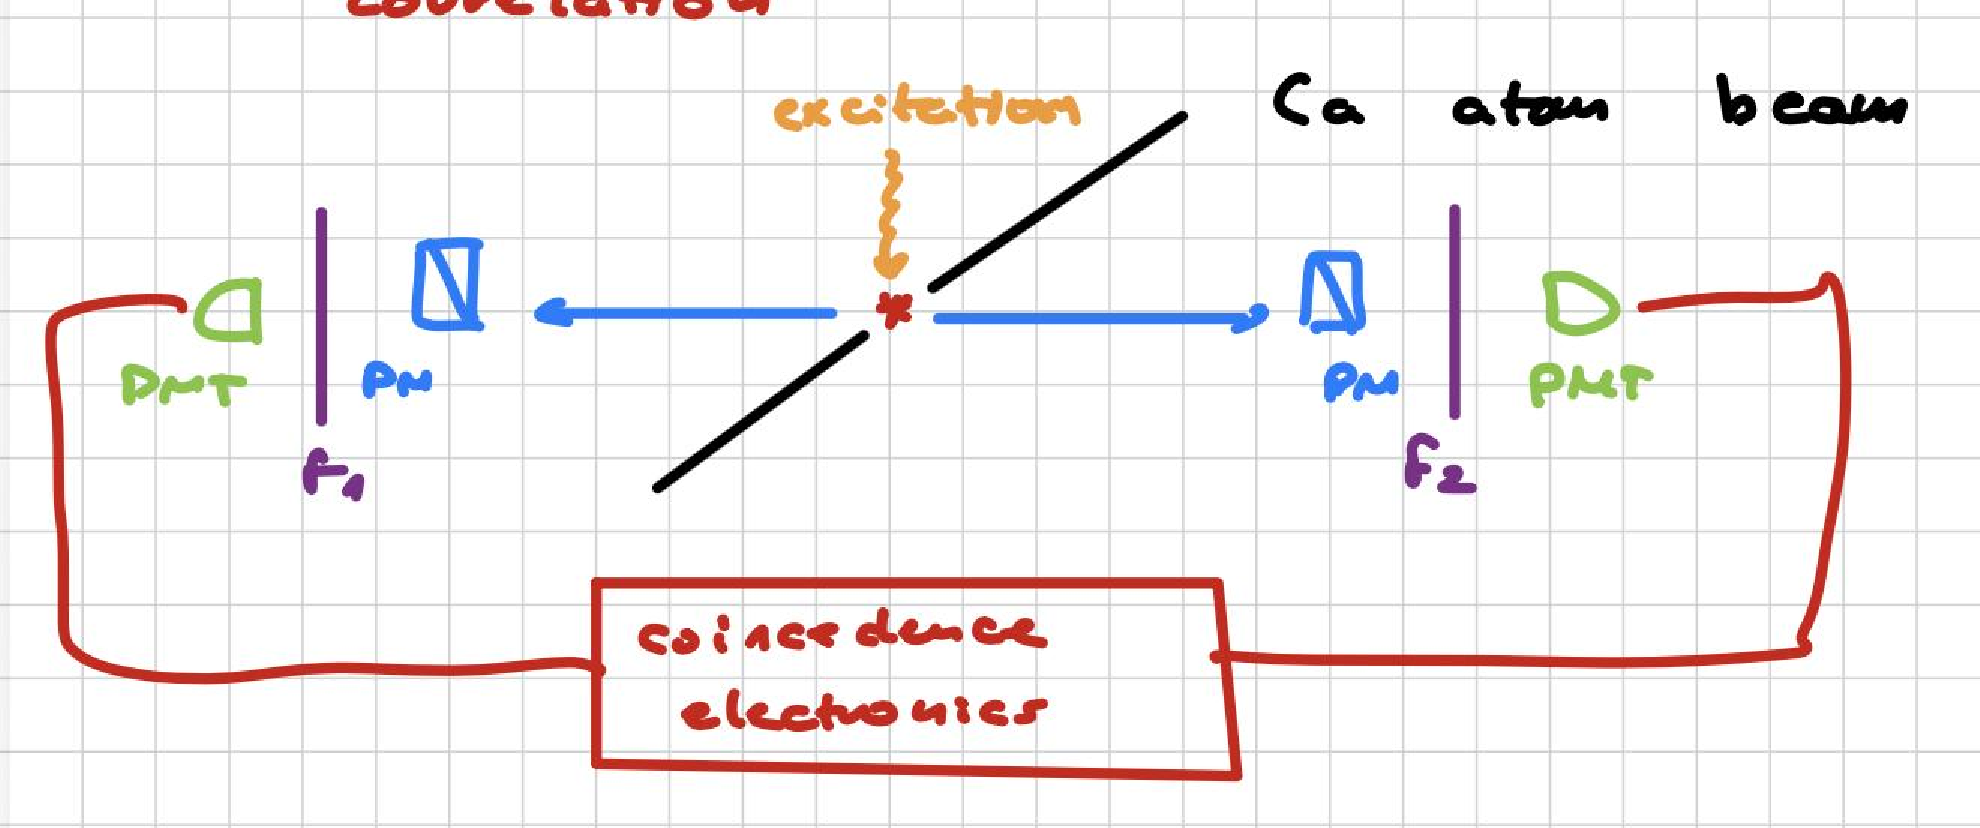
\includegraphics[width=0.6\linewidth]{images_in_pdf/15-/Grafico_84.pdf}
\end{figure}

A measurement along the $\vec{n}_A$ direction yields a vertical outcome $\ket{V}$ if the photon polarization is parallel to $\vec{n}_A$, or a horizontal outcome $\ket{H}$ if it is perpendicular. We can then define the experimental \textbf{correlation coefficient} $E(\vec{n}_A,\vec{n}_B)$ as:
\begin{equation}\label{eqn:15-correlation-coefficient}
E(\vec{n}_A,\vec{n}_B) = P_{VV}(\vec{n}_A,\vec{n}_B) + P_{HH}(\vec{n}_A,\vec{n}_B) - P_{VH}(\vec{n}_A,\vec{n}_B) - P_{HV}(\vec{n}_A,\vec{n}_B),
\end{equation}
where $P_{ij}$ represents the joint probability of detecting outcome $i$ at station A and outcome $j$ at station B.

To maximize the experimental violation, we consider a combination of four distinct polarizer orientations -- $\vec{n}_A, \vec{n}_A'$ for Alice and $\vec{n}_B, \vec{n}_B'$ for Bob -- grouped into the $\mathbf{S}$\textbf{-parameter}:
\begin{equation}\label{eqn:15-s-parameter}
S = E(\vec{n}_A,\vec{n}_B) + E(\vec{n}_A,\vec{n}_B') + E(\vec{n}_A',\vec{n}_B) - E(\vec{n}_A',\vec{n}_B').
\end{equation}

\hl{In any realistic local theory, this expression is bounded by the \textbf{CHSH inequality}} (Clauser-Horne-Shimony-Holt):
\begin{equation}\label{eqn:15-chsh-bounds}
-2 \leq S \leq 2.
\end{equation}

Conversely, quantum mechanics predicts that for polarization-entangled states, the correlation coefficient scales as 
\begin{equation}\label{eqn:15-quantum-correlation-2}
E(\phi) = \cos(2\phi), 
\end{equation}

where $\phi$ is the relative angle between the polarizers. If we choose a geometric configuration where the angular separations are $\theta_{AB} = \theta_{AB'} = \theta_{A'B} = \theta$, while the fourth pair is widely separated by $\theta_{A'B'} = 3\theta$, the $S$-parameter becomes a function of a single angle:
\begin{equation}\label{eqn:15-s-theta}
S(\theta) = 3\cos(2\theta) - \cos(6\theta).
\end{equation}

Maximizing this function at $\theta = \qty{22.5}{\degree}$ yields the maximum quantum mechanical violation known as the Cirel'son bound:
\begin{equation}\label{eqn:15-tsirelson-bound}
S = \pm 2\sqrt{2} \approx \pm 2.828,
\end{equation}
which \hl{heavily contradicts the local realistic limit of $2$}. Historical experiments (such as those by Alain Aspect) closely matched the quantum mechanical predictions, yielding an experimental value of:
\begin{equation}\label{eqn:15-experimental-s-chsh}
S_{\text{exp}} = 2.697 \pm 0.015 \qquad \text{at } \theta = \qty{22.5}{\degree},
\end{equation}

which \hl{rules out local hidden variables by many standard deviations}.

\begin{figure}[H]
    \centering
    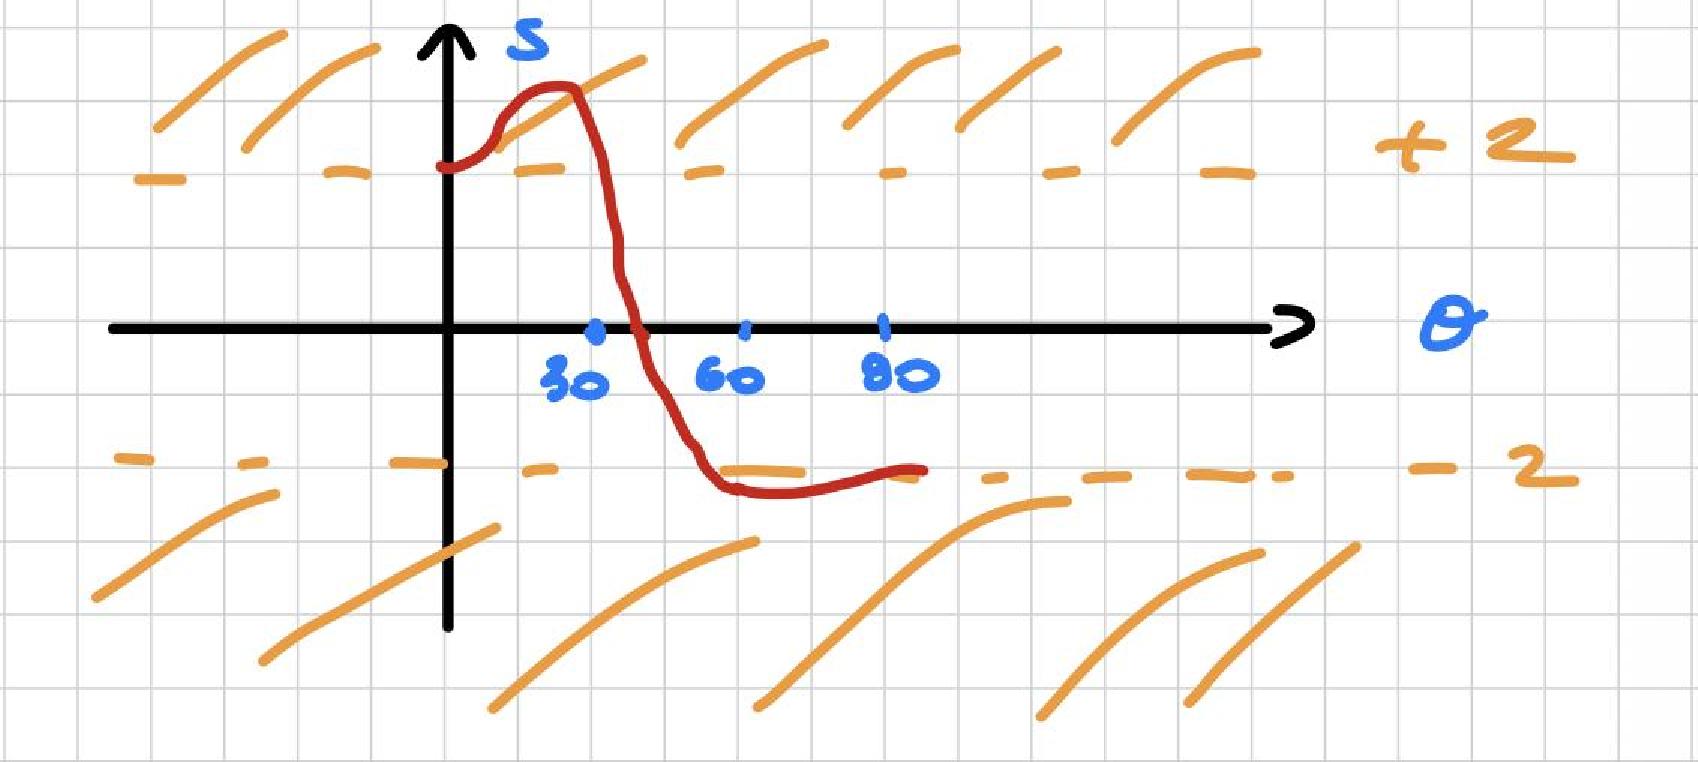
\includegraphics[width=0.6\linewidth]{images_in_pdf/15-/Grafico_85.pdf}
\end{figure}


\subsubsection{Loophole problems}
To ensure the validity of these experimental conclusions, one must address various \hl{experimental vulnerabilities, known as loopholes}, that could potentially allow for local hidden-variable explanations. The main loopholes are:

\begin{itemize}
    \item \textbf{Locality loophole:} There is a risk that the two measurement stations could exchange sub-luminal coordination signals during the photon flight time. To close this loophole, the setup can be upgraded by implementing high-speed acousto-optic modulators (AOMs). Driven by acoustic transducers, these devices switch the optical path between alternative polarizers on a timescale of $\sim \qty{20}{\nano\second}$. Since this switching time is much shorter than the light propagation time between the stations ($\Delta t \ll L/c$, where $L$ is the physical separation), the measurement settings are chosen at space-like separated intervals, preventing any causal communication.
    
    \item \textbf{Freedom-of-choice loophole:} This requires that the random generation of the analyzer settings must be completely independent of any properties or shared history of the entangled particle pair.
    
    \item \textbf{Detection loophole:} If the detectors sample only a small subset of the emitted pairs due to low quantum efficiency $\eta$, one could argue that the recorded events are biased and unrepresentative of the entire ensemble. Closing this loophole requires high-efficiency detectors; in a standard CHSH scenario, the symmetric detection efficiency threshold must satisfy $\eta \gtrsim 83\%$.
\end{itemize}

A fully loophole-free experimental demonstration -- simultaneously closing the locality, freedom-of-choice, and detection loopholes -- was successfully achieved in 2015. 

\calloutinfo{%
    Ultimately, Bell's theorem does not imply the existence of faster-than-light signaling, but rather demonstrates that \textbf{no local realistic theory can reproduce the non-local correlations of quantum mechanics}. Entangled photons do not carry predetermined local properties before a measurement is performed; their physical state is not fully encoded in pre-existing local variables, but is established contextually at the moment of detection.
}